\documentclass[final,5p,times,twocolumn,number,sort&compress]{elsarticle}

\usepackage{amssymb}
\usepackage{amsmath}
\usepackage{booktabs}
\usepackage{threeparttable}
\usepackage{makecell}
\usepackage{caption}
\usepackage[version=4]{mhchem}
\usepackage[hidelinks]{hyperref}
\usepackage[capitalise]{cleveref}

\newcommand{\hide}[1]{}

\journal{Physics Letters B}

\begin{document}

\begin{frontmatter}

\title{Distinct $\alpha$ Decay Branches in $^{273}$Ds and Evidence for a Low-Energy State in $^{269}$Hs near $N=162$}

\author{Z.\ R.\ Sun \hide{(孙志睿)}}
\affiliation{State Key Laboratory of Heavy Ion Science and Technology, Institute of Modern Physics, Chinese Academy of Sciences, Lanzhou 730000, China}
\affiliation{School of Nuclear Science and Technology, University of Chinese Academy of Sciences, Beijing 100049, China}

\begin{abstract}
A series of experiments was carried out at the SHANS-2 separator of IMP CAS to study the $^{238}$U($^{40}$Ar, $4n$--$5n$)$^{274,273}$Ds reaction. The excitation function was investigated in the excitation-energy range from 42 to 50 MeV. At 42 and 45 MeV, no correlated decay chain attributable to $^{273}$Ds was identified, and upper limits of 0.34 and 1.09 pb were obtained. At 50 MeV, two complete decay chains of $^{273}$Ds were observed, corresponding to a cross section of $0.14^{+0.18}_{-0.08}$ pb, in agreement with the value of $0.18^{+0.44}_{-0.12}$ pb reported previously for the same reaction at DGFRS-2. One chain follows the known high-energy, short-lived branch, whereas the other defines a lower-energy, longer-lived branch that supports the interpretation of a distinct state in $^{273}$Ds. By combining the present data with earlier results, the population pattern and the $\alpha$-particle energy distribution of $^{269}$Hs suggest the presence of an additional low-energy state in this nucleus. The combined decay properties and isotopic systematics of Ds and Hs provide new constraints on the single-particle structure around the deformed $N=162$ shell closure.
\end{abstract}

\begin{keyword}
$\alpha$ decay \sep $N=162$ subshell \sep Isomeric state \sep Gas-filled recoil separator
\end{keyword}

\end{frontmatter}

\section{Introduction}
\label{introduction}

In the absence of shell corrections, the macroscopic liquid-drop model does not allow the existence of superheavy elements ($Z \ge 104$), because the Coulomb repulsion becomes dominant. Nevertheless, major experimental and theoretical progress has enabled the synthesis of nuclei in this extreme mass region, in particular through $^{48}\mathrm{Ca}$-induced reactions \cite{oganessianSuperheavyNuclei48Cainduced2015,oganessianInvestigationCa482022}. The existence and survival of these nuclei rely on quantum shell effects, which provide the additional binding energy required to stabilize them against spontaneous fission. Theoretical models predict that these shell corrections generate islands of stability across the superheavy landscape. Enhanced stability is expected near the deformed doubly magic region around $Z = 108$ and $N = 162$ \cite{dvorakDoublyMagicNucleus2006}, and the shell stabilization is predicted to extend toward heavier spherical configurations near $N = 184$ and $Z = 114$--126, although the exact location remains model dependent \cite{kruppa2000ShellCorrectionsSuperheavy}. Odd-$A$ nuclei in this mass region provide stringent tests of these theoretical frameworks, because their decay properties are sensitive to the single-particle structure around the deformed $N = 162$ shell gap.

In this context, $^{273}\mathrm{Ds}$ and its daughter $^{269}\mathrm{Hs}$ form a particularly important pair. The nucleus $^{273}\mathrm{Ds}$ contains one neutron above the $N = 162$ gap, whereas $^{269}\mathrm{Hs}$ corresponds to one neutron hole below it. The $\alpha$-decay link between these two nuclei therefore probes the single-particle structure on both sides of the same deformed shell closure. The isotope $^{273}\mathrm{Ds}$ was first identified unambiguously at SHIP as an $\alpha$-decay descendant in cold-fusion reactions \cite{hofmann2002NewResultsElements}. In the $^{208}\mathrm{Pb}(^{70}\mathrm{Zn}, n)^{277}\mathrm{Cn}$ experiments at GSI \cite{hofmann2002NewResultsElements,hofmann1996NewElement112} and RIKEN \cite{sumita2013NewResultProduction,morita2007ExperimentSynthesisIsotope277}, the lifetime of the $^{273}\mathrm{Ds}$ descendant was consistently found in the $0.1\ \mathrm{ms}$ range. More recently, direct production of $^{273}\mathrm{Ds}$ in the $^{238}\mathrm{U}(^{40}\mathrm{Ar}, 5n)$ reaction was reported by Oganessian \textit{et al.} \cite{oganessian2024SynthesisDecayProperties}. Two genetically correlated decay chains were observed, one of which was interpreted as originating from an isomeric state of $^{273}\mathrm{Ds}$. However, those chains were incomplete and therefore provided only limited information on the decay of the daughter nucleus $^{269}\mathrm{Hs}$.

In the present work, the same reaction was studied at the SHANS-2 separator \cite{xu2023GasfilledRecoilSeparator}. Two additional complete decay chains were observed and assigned to $^{273}\mathrm{Ds}$ on the basis of genetic correlations \cite{geneticcorrelations} and consistency with historical data. These new data provide independent support for the existence of two distinct decay branches in $^{273}\mathrm{Ds}$, denoted here as $^{273}\mathrm{Ds}^{a}$ and $^{273}\mathrm{Ds}^{b}$ following Ref.~\cite{oganessian2024SynthesisDecayProperties}. By combining the present results with earlier measurements and with macroscopic--microscopic considerations, the present work examines the possible existence of isomeric structures in $^{273}\mathrm{Ds}$ and $^{269}\mathrm{Hs}$ and discusses the implications for the shell structure near $N = 162$.

\section{Experiment and results}

The experiment was performed at the China Accelerator Facility for Superheavy Elements of the Institute of Modern Physics by using the gas-filled recoil separator SHANS-2 (Spectrometer for Heavy Atoms and Nuclear Structure-2). The nucleus $^{273}\text{Ds}$ was synthesized in the $^{238}\text{U}(^{40}\text{Ar}, 5n)$ fusion-evaporation reaction. A $^{40}\text{Ar}^{13+}$ beam with average incident energies of 217, 220, and 225 MeV was delivered by the superconducting linear accelerator. The typical beam intensity on target was about $5\ \mathrm{p}\mu\mathrm{A}$, and the total effective irradiation time was about 728 h.

The targets were prepared by magnetron sputtering of $^{238}\text{U}$ onto Ti backings with thicknesses of 2.22 and 2.19 $\mu\text{g/cm}^{2}$, resulting in average $^{238}\text{U}$ layer thicknesses of 470 and 604 $\mu\text{g/cm}^{2}$. The arc-shaped target segments were mounted on a wheel with a diameter of 50 cm and rotated at 1500 rpm during irradiation in order to withstand the high beam load.

Evaporation residues were separated in flight from the primary beam and other reaction products by SHANS-2. The separator was filled with helium gas at a pressure of about 1 mbar, and the magnetic rigidity was optimized for the transmission of $^{273}\text{Ds}$. At the focal plane, the evaporation residues passed through two multi-wire proportional chambers (MWPCs) and were then implanted into a double-sided silicon strip detector (DSSD). The MWPCs were mounted about 20 cm upstream of the DSSD and operated with isobutane gas. They were used mainly to distinguish implantation events from decay events by combining time-of-flight information with time--position correlations and the trigger status of the MWPCs.

The DSSD has an active area of $128 \times 48\ \text{mm}^{2}$ and a thickness of 300 $\mu\text{m}$. The front side, defined as the $X$ plane, is segmented into 128 vertical strips, whereas the back side, defined as the $Y$ plane, is segmented into 48 horizontal strips. This geometry provides 6144 pixels and a position resolution of about 1 mm. Six single-sided silicon detectors were arranged upstream of the DSSD in a box-like geometry to detect $\alpha$ particles and spontaneous-fission fragments escaping from the front side of the DSSD. Each detector has a thickness of 500 $\mu\text{m}$ and an active area of $120 \times 63\ \text{mm}^{2}$. In addition, three silicon detectors with a thickness of 300 $\mu\text{m}$ were installed directly behind the DSSD as veto detectors in order to reject light particles punching through the focal-plane detector system. The entire silicon array was cooled to about $-30^{\circ}\text{C}$ with a circulating alcohol system to suppress thermal noise and improve the energy resolution. For full-energy $\alpha$ particles in the range from 5 to 9 MeV, the typical full width at half maximum of the DSSD was about 30 keV. The detection efficiency for $\alpha$ particles was about 87(6)\%. All detector signals were preamplified, shaped, and digitized with 14-bit analog-to-digital converters operated at 100 MHz in a triggerless mode. Further details of SHANS-2 and the detector system can be found in Refs.~\cite{xu2023GasfilledRecoilSeparator,sheng2021IonopticalDesignMultiparticle}.

The silicon detectors were calibrated with standard $\alpha$ sources (\ce{^{239}Pu}, \ce{^{241}Am}, and \ce{^{244}Cm}) and with the well-known $\alpha$-decay lines of \ce{^{218}Rn} \cite{SINGH2019405}, \ce{^{214}Po} \cite{ZHU20211a}, \ce{^{216}Po} \cite{WU20071057}, and \ce{^{217}At} \cite{KONDEV2018382}. The reference energies were taken from the evaluated \textit{Nuclear Data Sheets}. The transmission efficiency used for the cross-section evaluation was obtained from simulations performed according to the procedure described in Ref.~\cite{zhang2026MonteCarloSimulation}, yielding a value of 20\%. The experimental conditions and the measured cross sections are summarized in Table~\ref{tab:cross_sections}.

\begin{table}[htbp]
\centering
\captionsetup{font=small}
\caption{Target thicknesses of $^{238}$U, average projectile energies $\bar{E}_{\rm lab}$ at the middle of the target layers, corresponding average excitation energies $\bar{E}^{*}$ of the compound nucleus calculated from the mass tables of Refs.~\cite{myers1996NuclearPropertiesAccording,wang2021NUBASE2020EvaluationNuclear}, total beam doses, and measured cross sections $\sigma$ or upper limits for the $4n$ and $5n$ evaporation channels in the $^{40}$Ar + $^{238}$U reaction. Values separated by ``$|$'' correspond to measurements with two target thicknesses, and the beam doses are listed in the same order.}
\label{tab:cross_sections}
\begin{threeparttable}
\setlength{\tabcolsep}{3.5pt}
\renewcommand{\arraystretch}{1.08}
\small
\begin{tabular*}{\columnwidth}{@{\extracolsep{\fill}}cccccc@{}}
\toprule
\makecell[c]{Target thickness\\(mg/cm$^{2}$)} &
\makecell[c]{$\bar{E}_{\rm lab}^{\,a}$\\(MeV)} &
\makecell[c]{$\bar{E}^{*}$\\(MeV)} &
\makecell[c]{Beam dose\\($\times 10^{19}$)} &
\makecell[c]{$\sigma_{4n}$\\(pb)} &
\makecell[c]{$\sigma_{5n}$\\(pb)} \\
\midrule
$0.47\,|\,0.60$ & 225 & 50 & $2.28\,|\,2.96$ & $<0.15$ & $0.14^{+0.18}_{-0.08}$ \\
0.47 & 220 & 45 & 0.817 & $<1.1$ & $<1.1$ \\
0.60 & 217 & 42 & 2.04 & $<0.34$ & $<0.34$ \\
\bottomrule
\end{tabular*}
\begin{tablenotes}[flushleft]
\footnotesize
\item[a] The systematic uncertainty of the beam energy is 1 MeV.
\end{tablenotes}
\end{threeparttable}
\end{table}

\section{Results and discussion}

For the $^{238}\text{U}(^{40}\text{Ar}, xn)^{278-x}\text{Ds}$ reaction at an excitation energy of about 50 MeV, the $5n$ evaporation channel is expected to be the dominant channel \cite{oganessian2024SynthesisDecayProperties}. At this energy, two decay chains were observed. The full event information is shown in Fig.~\ref{fig:decay-chain}.

\begin{figure}
\centering

\includegraphics[width=0.4\textwidth]{decayChain.pdf}
\caption{Two complete decay chains assigned to $^{273}$Ds in the $^{238}$U($^{40}$Ar, $5n$)$^{273}$Ds reaction. For each chain, the energy of the evaporation residue and the corresponding $X/Y$ implantation position are given at the top, followed by the energies of the successive $\alpha$ decays and of the terminal spontaneous-fission event together with the correlation times between adjacent signals. Energies in parentheses indicate summed signals. The numbers written as subscripts after the energies denote the corresponding uncertainties in units of keV. The red entries mark the newly observed branch and the related tentative state assignment discussed in the present work.}
\label{fig:decay-chain}
\end{figure}

The energy and decay time of $\alpha_{1}$ in Chain 1 are consistent with the data obtained in the previous cold-fusion $^{208}\text{Pb}(^{70}\text{Zn}, n)^{277}\text{Cn}$ experiments at GSI \cite{hofmann2002NewResultsElements,hofmann1996NewElement112} and RIKEN \cite{sumita2013NewResultProduction,morita2007ExperimentSynthesisIsotope277}, as well as with the direct-production experiment on $^{238}\text{U}(^{40}\text{Ar}, 5n)^{273}\text{Ds}$ at JINR \cite{oganessian2024SynthesisDecayProperties}. The subsequent decay properties of $^{269}\text{Hs}$, which produce $\alpha_{2}$ and $\alpha_{3}$, and the terminal spontaneous fission of $^{261}\text{Rf}$ in both chains are also consistent with the decay data reported in Refs.~\cite{dvorakDoublyMagicNucleus2006,dullmannCm248Ne2008,dvorakObservation3Evaporation2008,graegerExperimentalStudy2382010,vonzweidorfEvidenceFormationSodium2004,habaProductionDecayProperties2011,habaProduction265Sg2012}. The detailed assignments are discussed below.

D\"ullmann \textit{et al.}~\cite{dullmannCm248Ne2008} proposed that $^{261}\text{Rf}$ populated by the $\alpha$ decay of $^{265}\text{Sg}$ has two states, $^{261}\text{Rf}^{a}$ and $^{261}\text{Rf}^{b}$. The existence and decay properties of these states were later confirmed by Haba \textit{et al.}~\cite{habaProductionDecayProperties2011} in the $^{248}\text{Cm}(^{22}\text{Ne}, 5n)^{265}\text{Sg}$ reaction. The state $^{261}\text{Rf}^{a}$ decays to $^{257}\text{No}$ by emission of an 8.28 MeV $\alpha$ particle with $T_{1/2} = 68$ s, whereas $^{261}\text{Rf}^{b}$ has $T_{1/2} = 2.6\ \text{s}$ and decays through an 18\% $\alpha$ branch with $E_{\alpha} = 8.51\ \text{MeV}$ and an 82\% spontaneous-fission branch \cite{habaProductionDecayProperties2011}. The terminal spontaneous-fission events observed in both chains of the present work are therefore attributed to $^{261}\text{Rf}^{b}$.

D\"ullmann \textit{et al.}~\cite{dvorakDoublyMagicNucleus2006} also suggested that the $\alpha$ decay of $^{269}\text{Hs}$ proceeds through two distinct $\alpha$-particle energies, $E_{\alpha} = 9.13$ and $8.95\ \text{MeV}$, which populate two corresponding states in the daughter nucleus, $^{265}\text{Sg}^{a}$ and $^{265}\text{Sg}^{b}$. These values match the observed $E_{\alpha_{2}}$ values in Chain 1 and Chain 2, respectively. The decay properties of $^{265}\text{Sg}^{a}$ and $^{265}\text{Sg}^{b}$ were established later by Haba \textit{et al.}~\cite{habaProduction265Sg2012} from high-statistics data for the $^{248}\text{Cm}(^{22}\text{Ne}, 5n)^{265}\text{Sg}$ reaction. The state $^{265}\text{Sg}^{a}$, with $T_{1/2} = 8.5\ \text{s}$, decays by an 8.84 MeV $\alpha$ transition to $^{261}\text{Rf}^{a}$ and $^{261}\text{Rf}^{b}$ with branching ratios of 91\% and 9\%, respectively. The state $^{265}\text{Sg}^{b}$, with $T_{1/2} = 14.4\ \text{s}$, decays by an 8.69 MeV $\alpha$ transition to $^{261}\text{Rf}^{a}$ and $^{261}\text{Rf}^{b}$ with branching ratios of 20\% and 80\%, respectively. Both chains observed in the present work are therefore assigned to the sequence $^{265}\text{Sg}^{b} \rightarrow {}^{261}\text{Rf}^{b}$.

The $E_{\alpha}$ and $T_{1/2}$ values for all decay chains involving \ce{^{273}Ds} are compiled and compared with the historical data in Fig.~\ref{fig:EalphaAndDecaytime}.

\begin{figure}
\centering

\includegraphics[width=0.48\textwidth]{EalphaAndDecaytime.pdf}
\caption{Compilation of the $E_{\alpha}$ values and decay-time distributions for the decay chains involving $^{273}$Ds, $^{269}$Hs, $^{265}$Sg, and $^{261}$Rf. Panels (a)--(d) show the measured $\alpha$-particle energies, and panels (e)--(h) show the corresponding distributions of $\log_{10}[t(\mathrm{ms})]$. The red, blue, green, and yellow histograms represent the data from IMP, JINR \cite{oganessian2024SynthesisDecayProperties}, RIKEN \cite{sumita2013NewResultProduction,morita2007ExperimentSynthesisIsotope277}, and GSI \cite{hofmann2002NewResultsElements,hofmann1996NewElement112}, respectively. The smooth curves in the decay-time panels are drawn according to Ref.~\cite{schmidt2000NewTestRandom}.}
\label{fig:EalphaAndDecaytime}
\end{figure}

\subsection{\texorpdfstring{Decay properties of $^{273}\mathrm{Ds}$}{Decay properties of 273Ds}}

As shown in Fig.~\ref{fig:EalphaAndDecaytime}, most events in the two chains observed in the present work agree with the historical data. The notable exception is one $^{273}\text{Ds}$ decay with $E_{\alpha} = 10.858(14)\ \text{MeV}$ and $\tau = 8.320\ \text{ms}$, which differs substantially from the higher-energy, shorter-lived decays observed at GSI and RIKEN and from the short-lived branch identified in the present work. In combination with the chain reported in Ref.~\cite{oganessian2024SynthesisDecayProperties} with $E_{\alpha} = 10.929(14)\ \text{MeV}$ and $\tau = 41.703\ \text{ms}$, this observation supports the existence of a lower-energy, longer-lived branch in $^{273}\text{Ds}$.

The nucleus $^{273}\text{Ds}$ has been populated in two ways: as the $\alpha$-decay daughter of $^{277}\text{Cn}$ in the cold-fusion $^{208}\text{Pb}(^{70}\text{Zn}, n)$ reaction at GSI \cite{hofmann2002NewResultsElements,hofmann1996NewElement112} and RIKEN \cite{sumita2013NewResultProduction,morita2007ExperimentSynthesisIsotope277}, and by direct production in the hot-fusion $^{238}\text{U}(^{40}\text{Ar}, 5n)$ reaction at JINR \cite{oganessian2024SynthesisDecayProperties} and in the present work. Two groups of decay properties are now observed. Following Ref.~\cite{oganessian2024SynthesisDecayProperties}, the lower-energy, longer-lived branch is denoted as $^{273}\text{Ds}^{a}$ and the higher-energy, shorter-lived branch is denoted as $^{273}\text{Ds}^{b}$. The available data indicate that population through the decay of $^{277}\text{Cn}$ favors the former branch, whereas direct production populates both branches. This pattern is consistent with the interpretation of $^{273}\text{Ds}^{a}$ as a distinct low-lying state, possibly of isomeric character.

\subsection{\texorpdfstring{Decay properties of $^{269}\mathrm{Hs}$}{Decay properties of 269Hs}}

T\"urler \textit{et al.}~\cite{turlerNuclearStructureReaction2012} pointed out that the reported $\alpha$-decay energies of $^{269}\text{Hs}$ in the range 9.17--9.25 MeV, observed as descendants of $^{277}\text{Cn}$ and $^{273}\text{Ds}$, are among the highest known for this nuclide. Two explanations were considered: energy summing with conversion electrons in the focal-plane detector, or the presence of long-lived states in $^{269}\text{Hs}$ similar to those already established in $^{265}\text{Sg}$ and $^{261}\text{Rf}$. When the present data are combined with the historical information, the $^{269}\text{Hs}$ events can be grouped into several energy regions. Following the notation of Ref.~\cite{oganessian2024SynthesisDecayProperties}, the state with $E_{\alpha} = 9.20(4)\ \text{MeV}$ and $T_{1/2} = 13^{+10}_{-4}\ \text{s}$ is denoted as $^{269}\text{Hs}^{a}$, and the state with $E_{\alpha} = 9.08(15)\ \text{MeV}$ and $T_{1/2} = 2.8^{+13.6}_{-1.3}\ \text{s}$ is denoted as $^{269}\text{Hs}^{b}$. The event observed in the present work with $E_{\alpha} = 8.915\ \text{MeV}$ and $\tau = 9.363\ \text{s}$ is assigned to an additional low-energy group denoted as $^{269}\text{Hs}^{c}$. Because the energy resolution of part of the historical data is limited, the distinction between $^{269}\text{Hs}^{a}$ and $^{269}\text{Hs}^{b}$ is not always robust, and these two groups are combined as $^{269}\text{Hs}^{a+b}$ when appropriate.

\begin{figure}
\centering
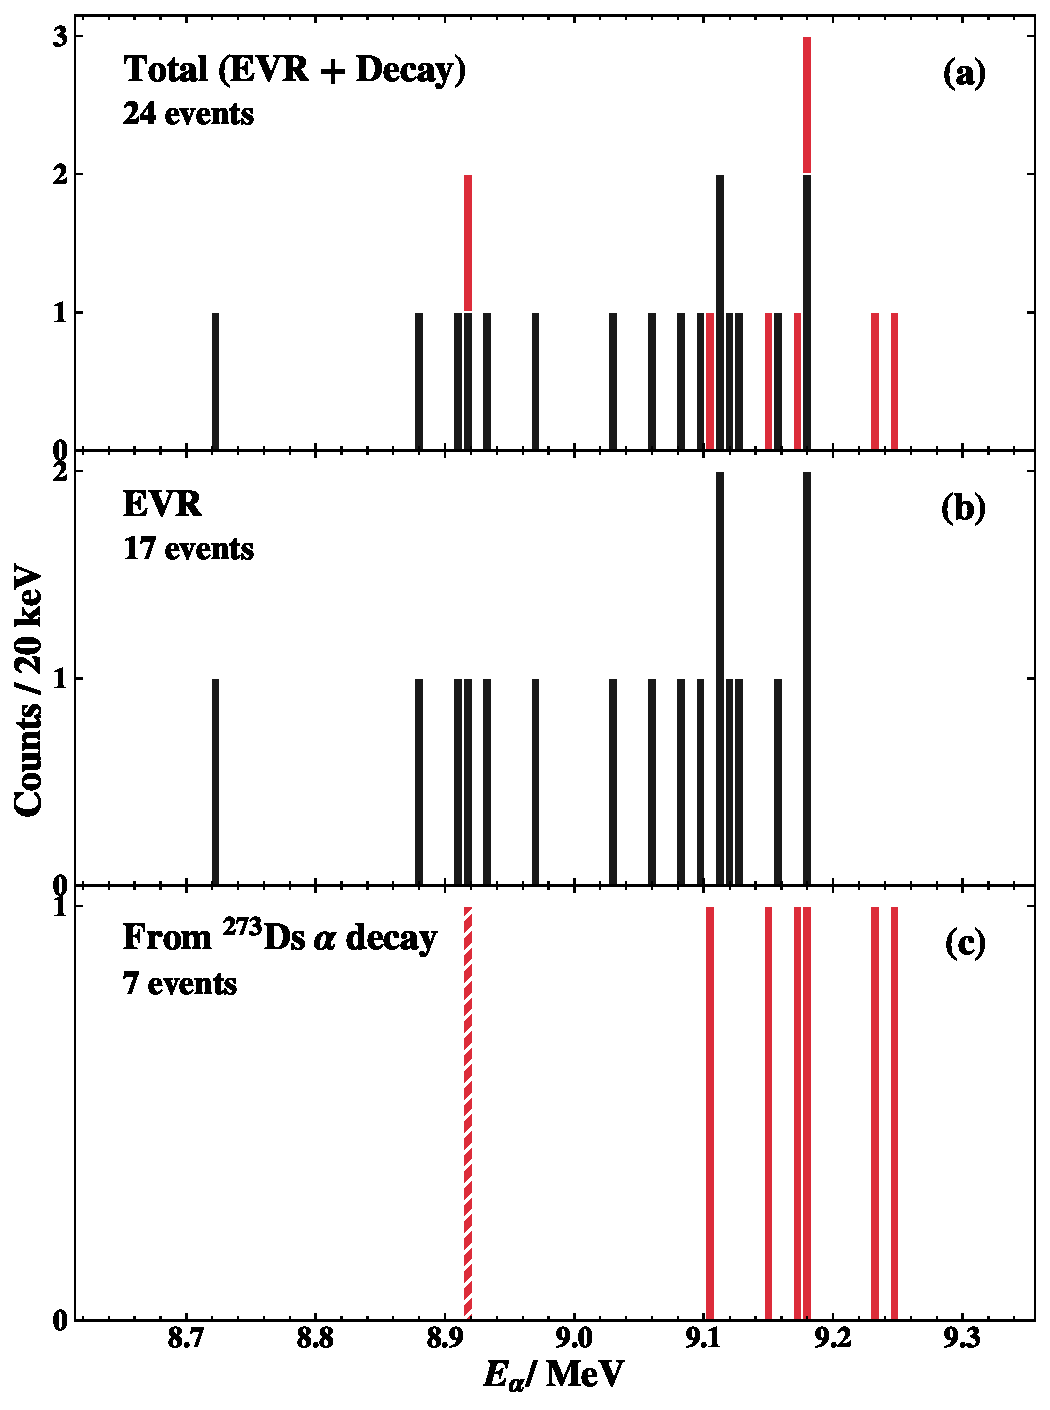
\includegraphics[width=0.4\textwidth]{distributionHs.pdf}
\caption{Measured $\alpha$-particle energy distribution for events assigned to $^{269}$Hs. Panel (a) shows the full event sample, panel (b) shows the directly produced evaporation-residue sample, and panel (c) shows the events populated through the $\alpha$ decay of $^{273}$Ds. The hatched bar marks the low-energy event observed in the present work at $E_{\alpha} = 8.915\ \text{MeV}$.}
\label{fig:distributionHs}
\end{figure}

As shown in Fig.~\ref{fig:distributionHs}, the directly produced $^{269}\text{Hs}$ events are distributed over both the high-energy and low-energy groups. By adopting 9.0 MeV as a practical dividing line, the event numbers in the present grouping correspond to $n(^{269}\text{Hs}^{a+b}):n(^{269}\text{Hs}^{c}) = 11:5$ for the directly produced sample and to $6:1$ for the sample populated through the $\alpha$ decay of $^{273}\text{Ds}$. These ratios are quoted directly from the full event compilation shown in Fig.~\ref{fig:distributionHs}, in which the questionable literature datum is retained for completeness. Within the present statistics, the low-energy group appears to be preferentially connected with the longer-lived branch of $^{273}\text{Ds}$, whereas no convincing example of the cross-population channels $^{273}\text{Ds}^{b} \rightarrow {}^{269}\text{Hs}^{c}$ or $^{273}\text{Ds}^{a} \rightarrow {}^{269}\text{Hs}^{a+b}$ is found. This selectivity suggests that $^{269}\text{Hs}^{c}$ may represent an additional low-lying state in $^{269}\text{Hs}$, although firmer support will require both higher-statistics data and dedicated structure calculations.

\section{Discussion}

For clarity, the working assignments adopted in the present work are summarized in Table~\ref{tab:state_summary}. On the basis of the present data, two distinct states are discussed for $^{273}$Ds, denoted as $^{273}$Ds$^{a}$ and $^{273}$Ds$^{b}$. By combining the present results with the data of Oganessian \textit{et al.}~\cite{oganessian2024SynthesisDecayProperties}, three groups are tentatively discussed for $^{269}$Hs, denoted as $^{269}$Hs$^{a}$, $^{269}$Hs$^{b}$, and $^{269}$Hs$^{c}$. At the present stage, the distinction between $^{269}$Hs$^{a}$ and $^{269}$Hs$^{b}$ remains less secure than the separation of $^{269}$Hs$^{c}$, because the statistics are limited and part of the historical data has a modest energy resolution. The present classification should therefore be regarded as a working scheme for discussing the decay pattern and the underlying structure rather than as a definitive level assignment.

\begin{table}[htbp]
\centering
\caption{Working assignment of the decay branches discussed in the present work. The labels $a$, $b$, and $c$ are descriptive identifiers used for discussion and do not imply definitive spin-parity assignments.}
\label{tab:state_summary}
\setlength{\tabcolsep}{3pt}
\renewcommand{\arraystretch}{1.08}
\small
\begin{tabular*}{\columnwidth}{@{\extracolsep{\fill}}p{0.18\columnwidth}p{0.28\columnwidth}p{0.30\columnwidth}p{0.18\columnwidth}@{}}
\toprule
State & Characteristic signature & Adopted decay branch & Status \\
\midrule
$^{273}\mathrm{Ds}^{b}$ & higher $E_{\alpha}$ and shorter lifetime & $^{273}\mathrm{Ds}^{b} \rightarrow {}^{269}\mathrm{Hs}^{a+b} \rightarrow {}^{265}\mathrm{Sg}^{b} \rightarrow {}^{261}\mathrm{Rf}^{b}$ & supported by present work and literature \\
$^{273}\mathrm{Ds}^{a}$ & lower $E_{\alpha}$ and longer lifetime & $^{273}\mathrm{Ds}^{a} \rightarrow {}^{269}\mathrm{Hs}^{c} \rightarrow {}^{265}\mathrm{Sg}^{b} \rightarrow {}^{261}\mathrm{Rf}^{b}$ & tentative low-lying or isomeric branch \\
$^{269}\mathrm{Hs}^{a}$ & $E_{\alpha}$ around 9.20 MeV and longer lifetime & feeds $^{265}\mathrm{Sg}^{b}$ through the high-energy group & historical assignment \\
$^{269}\mathrm{Hs}^{b}$ & $E_{\alpha}$ around 9.08 MeV and shorter lifetime & feeds $^{265}\mathrm{Sg}^{b}$ through the high-energy group & historical assignment \\
$^{269}\mathrm{Hs}^{c}$ & $E_{\alpha} = 8.915\ \mathrm{MeV}$ and intermediate lifetime & preferentially linked with $^{273}\mathrm{Ds}^{a}$ in the present scheme & tentative additional low-energy state \\
\bottomrule
\end{tabular*}
\end{table}

The most direct result of the present work is the appearance of two distinct decay patterns in $^{273}$Ds. One branch is characterized by a higher $\alpha$-decay energy and a shorter lifetime, whereas the other branch shows a lower $\alpha$-decay energy and a much longer lifetime. When the present chains are considered together with the chain reported in Ref.~\cite{oganessian2024SynthesisDecayProperties}, this separation is difficult to reconcile with a single-state interpretation. At the same time, the decay pattern of $^{269}$Hs is not random. The high-energy and low-energy groups are not populated with the same weight in direct production and in the decay of $^{273}$Ds, and the data do not show obvious cross feeding between the two proposed parent branches and the daughter groups. Such selectivity is naturally suggestive of configuration-dependent $\alpha$ decay.

Accordingly, the branch that starts from the higher $E_{\alpha}$ value and the shorter lifetime of $^{273}\mathrm{Ds}$ is assigned to
\begin{align*}
^{273}\text{Ds}^{b} &\xrightarrow{\alpha} {}^{269}\text{Hs}^{a,b} \xrightarrow{\alpha} {}^{265}\text{Sg}^{b} \xrightarrow{\alpha} {}^{261}\text{Rf}^{b} \xrightarrow{\text{SF}} \text{fission} .
\end{align*}
The branch that starts from the lower $E_{\alpha}$ value and the longer lifetime of $^{273}\mathrm{Ds}$ is assigned to
\begin{align*}
^{273}\text{Ds}^{a} &\xrightarrow{\alpha} {}^{269}\text{Hs}^{c} \xrightarrow{\alpha} {}^{265}\text{Sg}^{b} \xrightarrow{\alpha} {}^{261}\text{Rf}^{b} \xrightarrow{\text{SF}} \text{fission} .
\end{align*}

A plausible physical interpretation is that the long-lived branch of $^{273}$Ds is associated with a structure different from that of the short-lived branch. In a strongly deformed odd-$N$ nucleus, the $\alpha$-decay rate is controlled not only by $Q_{\alpha}$, but also by the angular-momentum change, the overlap between the initial and final intrinsic configurations, and the corresponding hindrance of $\alpha$ formation and barrier penetration \cite{clark2023RoleQuasiparticleStructure}. A large difference in lifetime between two branches of the same nuclide can therefore arise even when the difference in $Q_{\alpha}$ is modest. In this context, the observed separation between $^{273}$Ds$^{a}$ and $^{273}$Ds$^{b}$ is consistent with the presence of two competing quasineutron configurations, one of which gives rise to a hindered and longer-lived $\alpha$ decay.

\begin{figure*}[t]
\centering
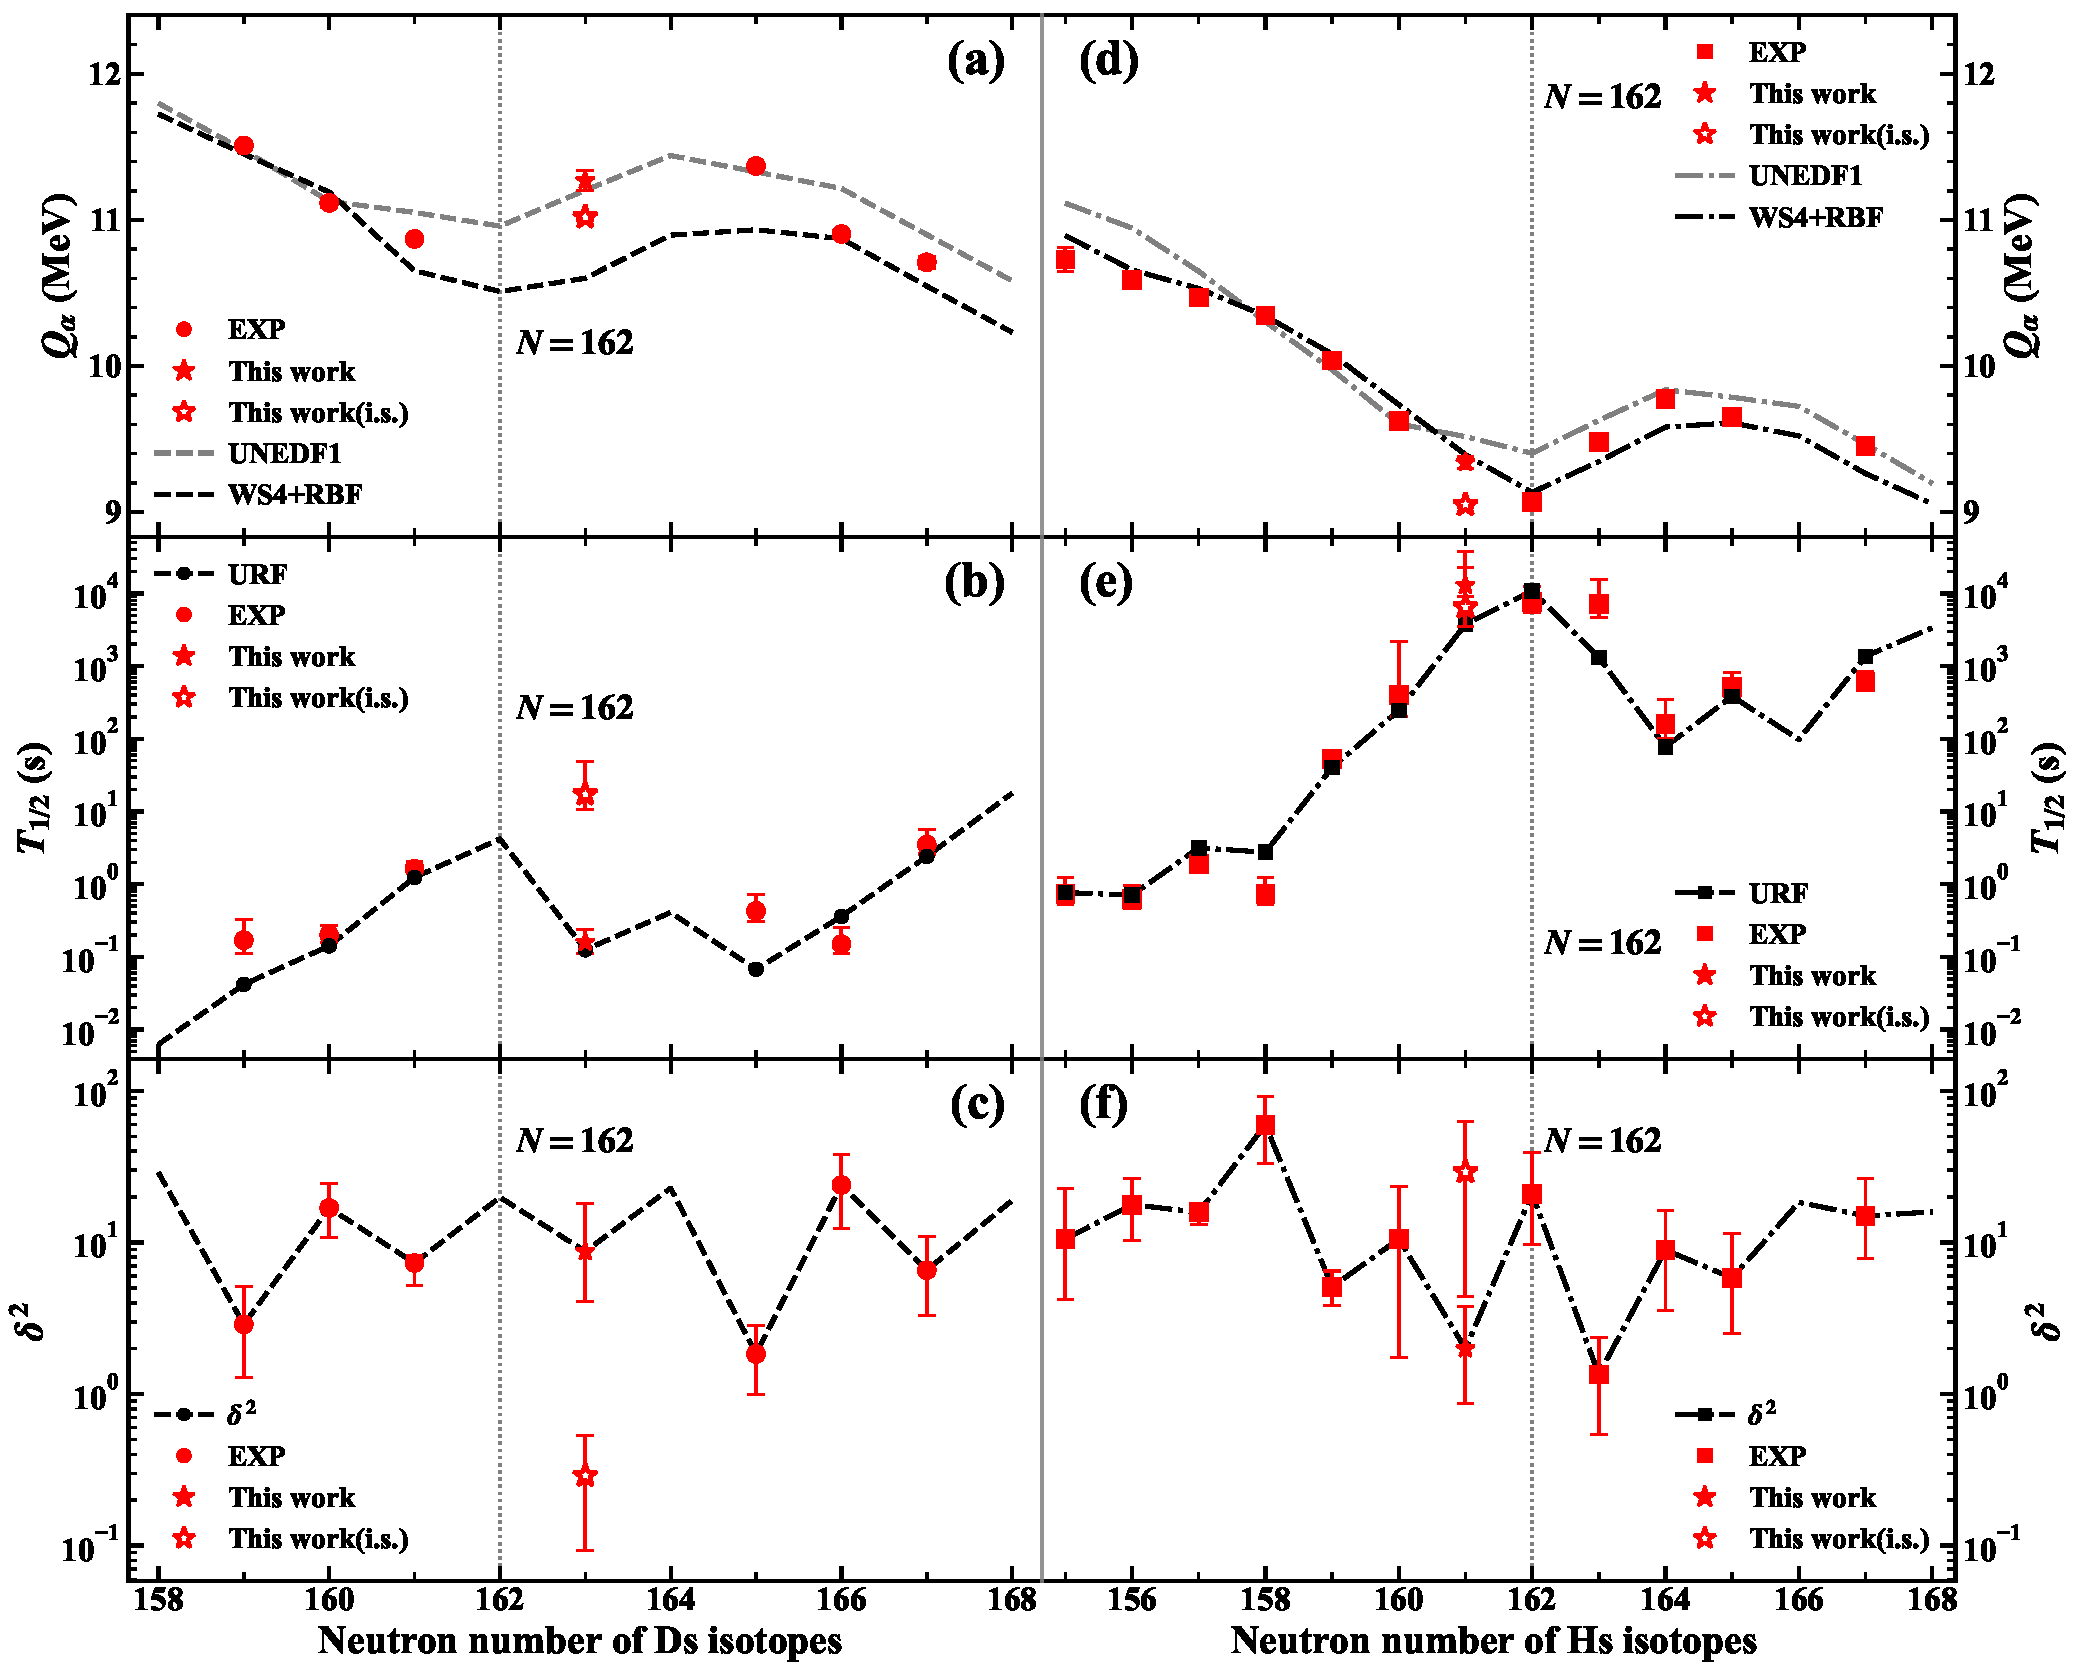
\includegraphics[width=1\textwidth]{System.pdf}
\caption{Systematics of $Q_{\alpha}$, $T_{1/2}$, and reduced $\alpha$-decay width $\delta^{2}$ for the Ds and Hs isotopic chains. Panels (a)--(c) correspond to Ds isotopes and panels (d)--(f) correspond to Hs isotopes. The upper, middle, and lower rows show $Q_{\alpha}$, $T_{1/2}$, and $\delta^{2}$, respectively, as functions of neutron number. Experimental values are compared with the UNEDF1 and WS4+RBF calculations in the $Q_{\alpha}$ panels and with the URF values in the half-life panels. The filled stars denote the branches assigned in the present work, and the open stars denote the tentative isomeric branches. The vertical dotted lines indicate $N=162$.}
\label{fig:System}
\end{figure*}

This interpretation is especially interesting in view of the expected shell structure around the deformed $N = 162$ gap \cite{guoStabilizationDeformedSuperheavy2024}. The nucleus $^{273}$Ds contains one neutron above this gap, whereas $^{269}$Hs corresponds to one neutron hole below it. The decay chain $^{273}$Ds $\rightarrow$ $^{269}$Hs therefore probes the single-particle structure on both sides of the same deformed shell closure. Several theoretical calculations indicate that low-lying high-$\Omega$ neutron configurations may be important in this region. In particular, the unique-parity orbital $\nu 13/2^{-}[716]$ has been predicted to lie close to the Fermi surface, while macroscopic--microscopic calculations for neighboring odd-$N$ transfermium nuclei also place $\nu 11/2^{-}[725]$ among the low-lying candidates \cite{Shi2014,Parkhomenko2005}. Within this picture, the long-lived branch of $^{273}$Ds may be associated with a high-$\Omega$ one-neutron configuration. This possibility is qualitatively consistent with the occurrence of high-$K$ isomerism in the neighboring deformed superheavy region, as discussed for the $^{270}$Ds $\rightarrow$ $^{266}$Hs decay sequence \cite{xuEnhancedStabilitySuperheavy2004}. At present, however, the available data do not allow a unique spin-parity or Nilsson-orbital assignment, and several interpretations remain possible.

Within the same framework, the decay selectivity observed in the daughter nucleus $^{269}$Hs also acquires a natural interpretation. If $^{273}$Ds$^{a}$ and $^{273}$Ds$^{b}$ correspond to different intrinsic configurations, favored $\alpha$ decay is expected to populate daughter states with similar structure. The proposed $^{269}$Hs$^{c}$ group, which appears in the low-energy branch and is preferentially associated with $^{273}$Ds$^{a}$, may therefore reflect a corresponding low-lying configuration in the daughter nucleus. By contrast, the higher-energy groups $^{269}$Hs$^{a}$ and $^{269}$Hs$^{b}$ may be associated with the decay of $^{273}$Ds$^{b}$. In this sense, the present data may indicate not only a possible isomeric structure in $^{273}$Ds, but also a correlated multistate structure in $^{269}$Hs. It should nevertheless be emphasized that the present evidence for three distinct groups in $^{269}$Hs remains tentative, and the possibility that part of the observed pattern reflects unresolved subgroups cannot yet be excluded.

Additional support for this picture is provided by the isotopic systematics. As shown in Fig.~\ref{fig:System}, the evolution of $Q_{\alpha}$, half-life, and reduced $\alpha$-decay width along the Ds and Hs isotopic chains gives a broader context for the present assignments. In a simple single-configuration picture, these observables are expected to change rather smoothly with neutron number. A local separation of branches, especially when it appears simultaneously in decay energy, lifetime, and reduced width, is more naturally interpreted as a signature of a structural change than as a statistical fluctuation. In the present case, the long-lived branch of $^{273}$Ds and the low-energy branch of $^{269}$Hs deviate from the local trends and therefore strengthen the interpretation in terms of different underlying configurations. At the same time, the reduced width in this strongly deformed superheavy region is model dependent, because deformation, angular-momentum change, and structure effects all enter its extraction. For this reason, the reduced width should not be regarded as a standalone proof of isomerism in the present work. Its main value is comparative: when it is evaluated consistently within the same prescription, it provides an additional indicator that the proposed branches are structurally different.

\begin{figure}
\centering
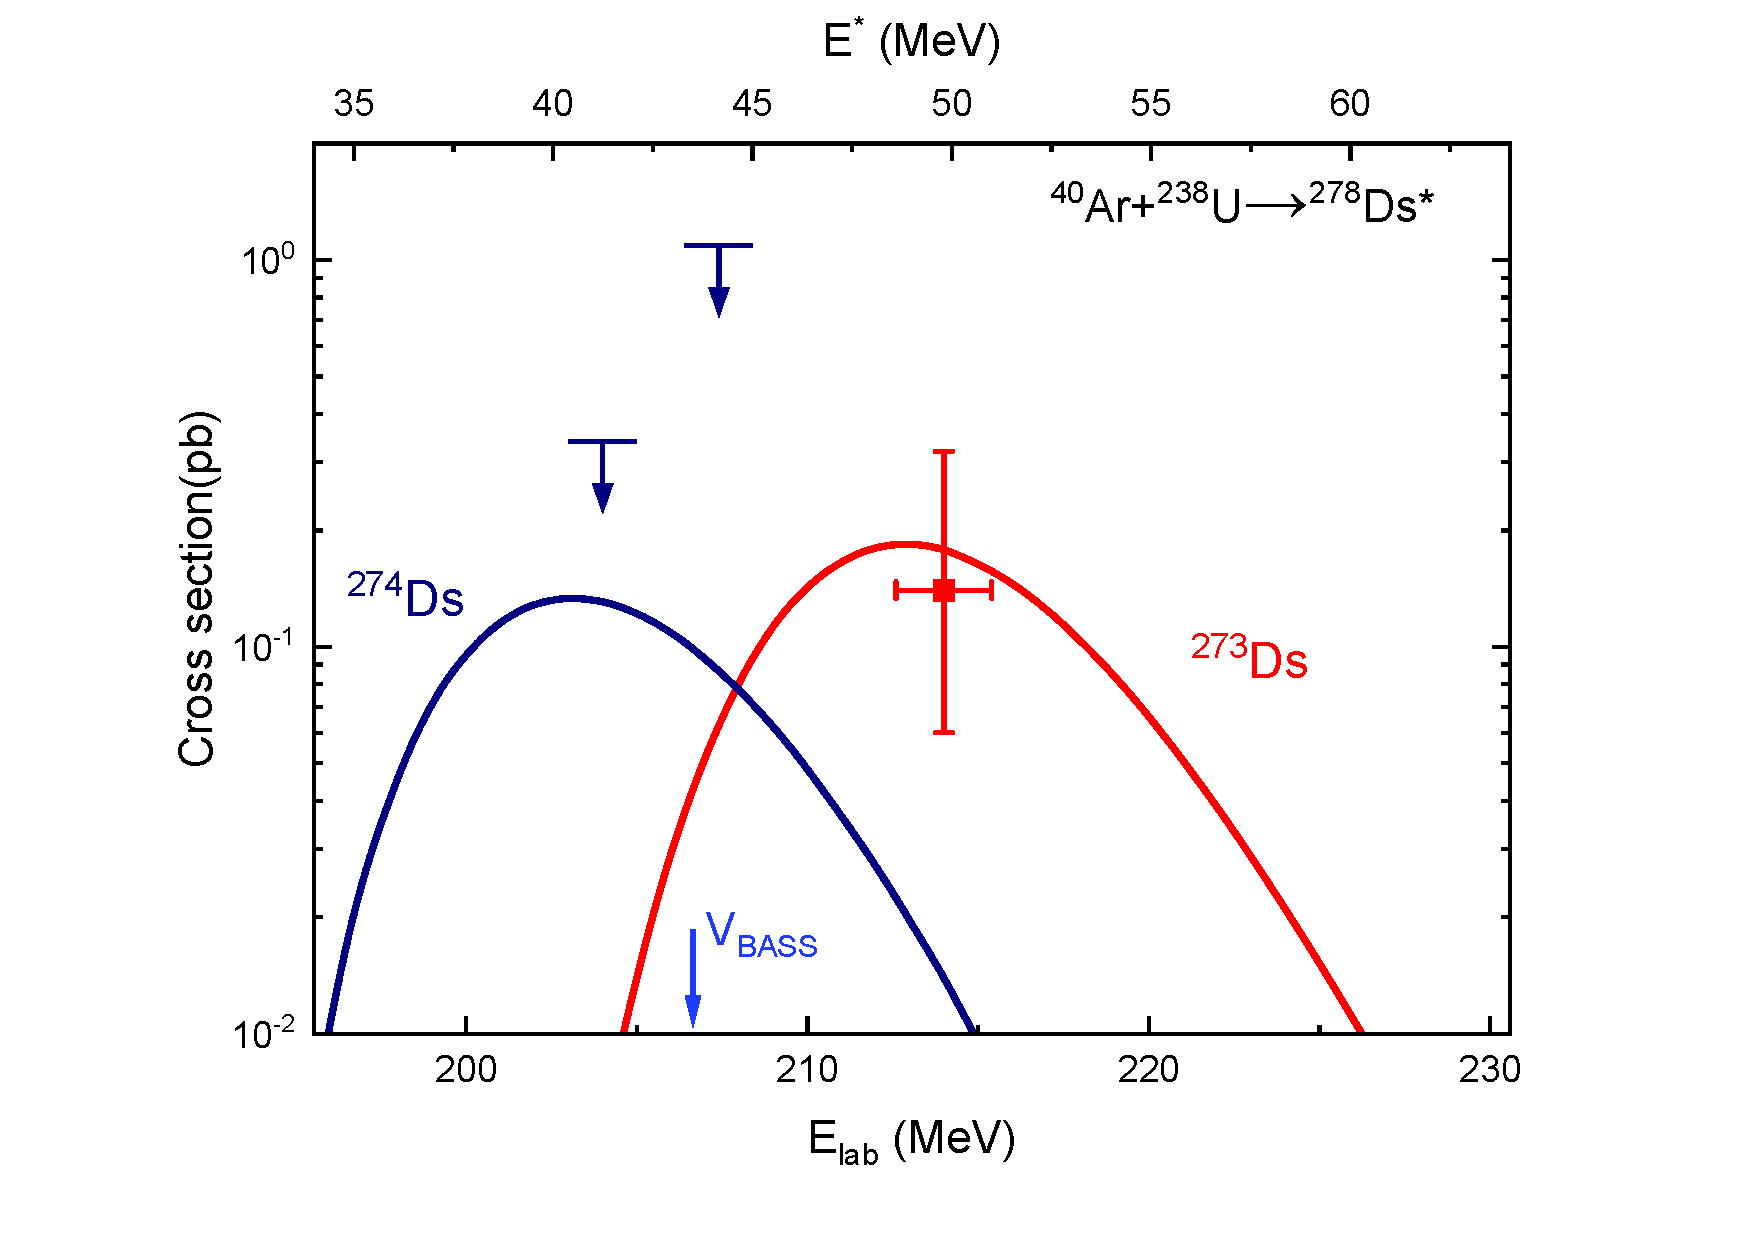
\includegraphics[width=0.5\textwidth]{exFun.pdf}
\caption{Measured cross section and upper limits for the $^{40}$Ar + $^{238}$U $\rightarrow$ $^{278}$Ds$^{*}$ reaction. The curves show the calculated excitation functions for the $4n$ and $5n$ channels leading to $^{274}$Ds and $^{273}$Ds, respectively. The lower horizontal axis gives the laboratory beam energy, and the upper axis gives the corresponding average excitation energy of the compound nucleus. The arrow marked $V_{\mathrm{BASS}}$ indicates the Coulomb barrier estimated with the BASS prescription.}
\label{fig:exFun}
\end{figure}

The excitation-function information provides an additional consistency check for the present interpretation. As shown in Fig.~\ref{fig:exFun}, the measured cross section at the present beam energy is broadly consistent with the calculated expectation that the $5n$ channel dominates near this energy. This agreement supports the assignment of the observed chains to $^{273}$Ds produced in the $^{238}$U($^{40}$Ar, $5n$)$^{273}$Ds reaction rather than to neighboring evaporation channels. Although the excitation function does not by itself distinguish between different intrinsic states, it shows that the long-lived and short-lived branches emerge within the same reaction framework. This point strengthens the conclusion that the difference between the two branches is more likely to be structural than to originate from different reaction channels.

\section{Summary and conclusions}

A beam-energy scan of the $^{238}$U($^{40}$Ar, $4n$--$5n$)$^{274,273}$Ds reaction was performed at SHANS-2. No correlated decay chain attributable to $^{273}$Ds was identified at excitation energies of 42 and 45 MeV, and upper limits of 0.34 and 1.09 pb were obtained. At 50 MeV, two complete decay chains of $^{273}$Ds were observed, and the extracted cross section of $0.14^{+0.18}_{-0.08}$ pb agrees with the value reported previously for the same reaction at DGFRS-2.

One of the observed chains follows the known high-energy, short-lived branch of $^{273}$Ds, whereas the other reveals a lower-energy, longer-lived branch. When the present data are combined with the literature results, the evidence supports the existence of two distinct decay branches in $^{273}$Ds, and the lower-energy branch is naturally interpreted as a candidate low-lying or isomeric state.

The daughter nucleus $^{269}$Hs shows a nonuniform population pattern. In addition to the previously recognized high-energy groups, the present work identifies a low-energy event at 8.915 MeV that is preferentially connected with the longer-lived branch of $^{273}$Ds. Although the present statistics remain limited, this behavior is compatible with the presence of an additional low-lying state in $^{269}$Hs.

The isotopic systematics of $Q_{\alpha}$, $T_{1/2}$, and reduced $\alpha$-decay width in the Ds and Hs chains provide further support for a structural change near $N = 162$. The overall picture is consistent with configuration-dependent $\alpha$ decay in odd-$N$ transfermium nuclei and provides new constraints on the ordering of low-lying quasineutron orbitals around the deformed $N = 162$ shell gap. More decisive conclusions will require higher-statistics direct-production measurements and dedicated structure calculations.

\section*{Acknowledgements}

The author thanks the operating staff of CAFE2 and SHANS-2 for stable beam delivery and technical support.

\bibliographystyle{elsarticle-num}
\bibliography{example}

\end{document}